\documentclass[pdf]
{beamer}
\mode<presentation>{}

\usepackage{amsmath}
\usepackage{tikz}
\usetikzlibrary{calc}                   
   

\newcommand\bayeseq{\mathrel{\overset{\makebox[0pt]{\mbox{\normalfont\tiny\sffamily Bayes}}}{=}}}

%% preamble
\title{Model inference from protein time-course in Hematopoietic Stem Cells (HSC)}
\subtitle{}
\author[shortname]{Quirin Heiss\inst{1, 2} \and Rene Schoeffel \inst{1, 2} \and Michael Strasser \inst{3}}
\institute[shortinst]{\inst{1} Technische Universit\"at M\"unchen \and %
                      \inst{2} Ludwig-Maximilians-Universit\"at M\"unchen \and %
                      \inst{2} Institute of Computational Biology (ICB), Helmholtz Zentrum M\"unchen}
\begin{document}

%% title frame
\begin{frame}
\titlepage
\end{frame}

%% normal frame
\begin{frame}{Introduction}
	\begin{itemize}
		\item Dynamics of hematopoetic stem cell lineage decision from Common Myeloid Progenitor (CMP) to Megakaryocyte-Erythroid Progenitor (MEP) and Granulocyte-Macrophage Progenitor (GMP) is our focus.
	\end{itemize}
	
	\begin{figure}[ht]
		\begin{center}
			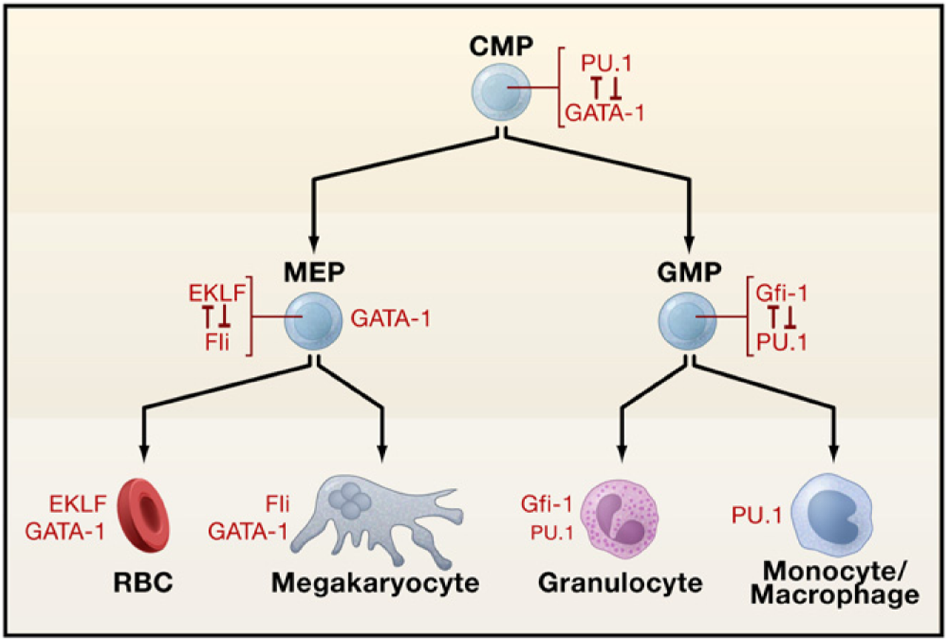
\includegraphics[height=2in]{figures/homatopoietic_focus.png}
			~\footnote{Graf \& Enver, 2009, \textit{Nature}}
		\end{center}
	\end{figure}
\end{frame}

\begin{frame}{Introduction (cont'd)}
	\begin{itemize}
		\item Assumed corss-inhibition dynamics between transcription factors \texttt{Pu.1} and \texttt{Gata1} in cell maturation fate:
	\begin{itemize}
		\item Dynamics is assumed to be a bistable toggle-switch system
		\item Lineage decision is a stochastics process resulting in uneven yield of MEP and GMP (70\% : 30\%)
	\end{itemize}
	\item Analysis on single-cell time-lapsed data to infer parameters of this dynamics.
	\end{itemize}
	\begin{figure}[ht]
		\begin{center}
			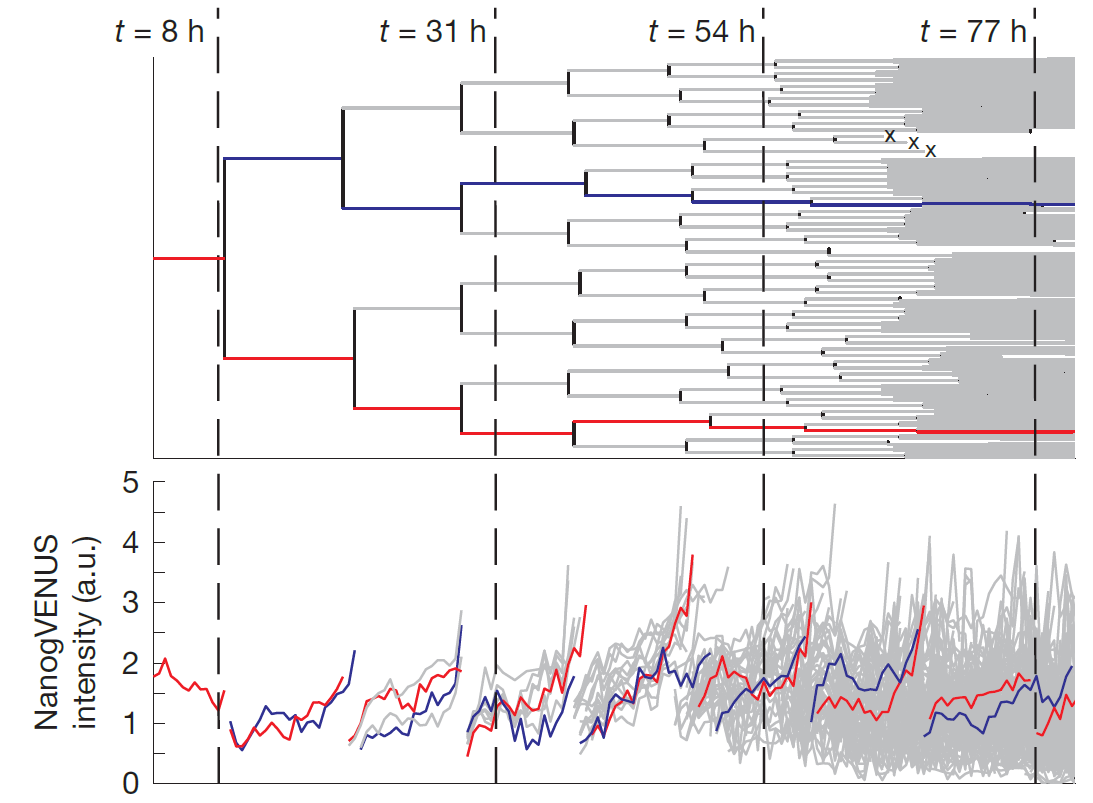
\includegraphics[height=1.5in]{figures/cell-generations.png}
			~\footnote{Feigelman, 2016, Ph.D. Thesis}
		\end{center}
	\end{figure}
\end{frame}

\begin{frame}{Problems}
	\textbf{Stochasticity of the system}
	\begin{itemize}
	\item Biophysical reaction is stochastic: reaction mechanism is inherently non-deterministic.
	\item Single cell analysis exposes stochasticity of the system: deterministic approaches not suitable in this case
	\end{itemize}
	\textbf{Branched data set}\\
	Tree structure of the data add more complexity: inheritance of information during inference process is not trivial
	
	\begin{figure}[ht]
		\begin{center}
			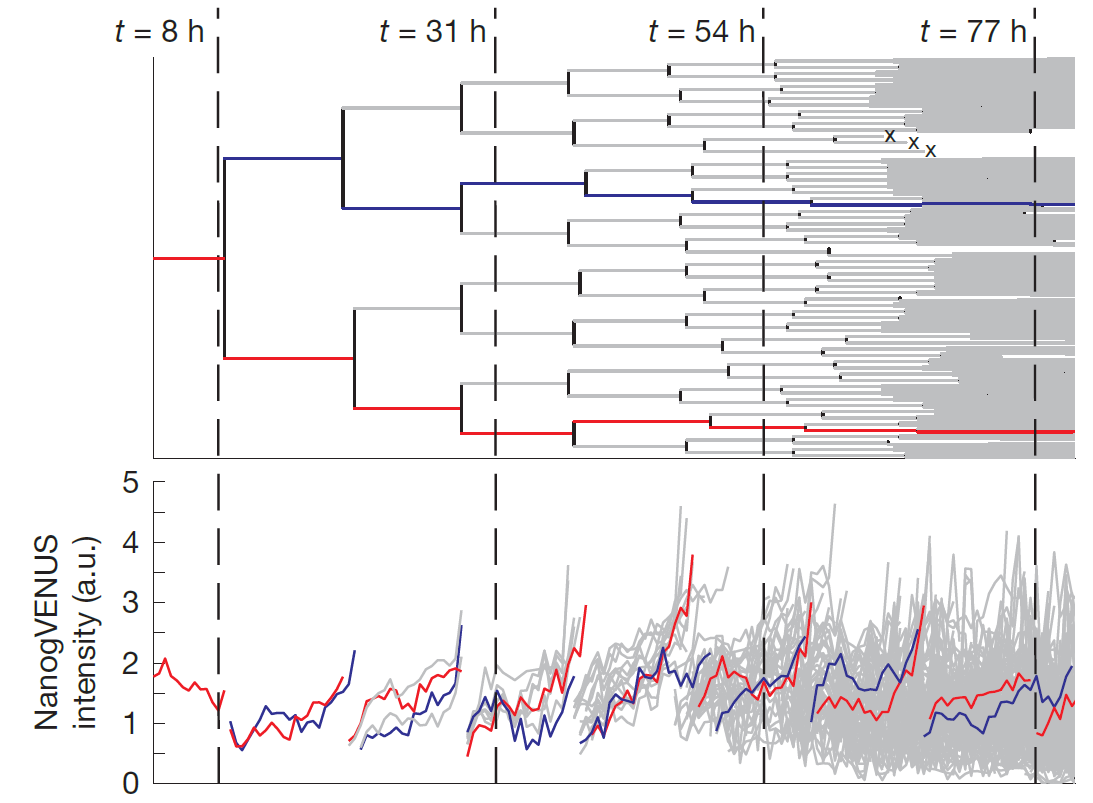
\includegraphics[height=1.5in]{figures/cell-generations.png}
			~\footnote{Feigelman, 2016, Ph.D. Thesis}
		\end{center}
	\end{figure}
\end{frame}

\begin{frame}{Ideas}
	\begin{itemize}
	\item Sequential Monte Carlo simulations using Gillespie algorithm along the time-lapsed data to infer sound parameters.
	\item<2-> \textbf{problem:} Overfitting due to single-cell biased.
	\item<3-> \textbf{solution:} Inference across cell lineages.
	\item<4-> Inferred parameters from all simulated lineages are represented as distribution.
	\item<5-> Final inferred parameters are expected value $E$ of the distribution.
	\end{itemize}
\end{frame}

\begin{frame}{Particle Filtering}

	\begin{itemize}

	\item \textbf{Particle}\\
	A particle K is defined as a triple of previous simulation trajectory $X$, parameter set $\theta$ and
assumed model $M$,

		\begin{equation}
		K := (X, \theta, M)
		\end{equation}
		
	\item \textbf{Particle filtering} is an parameters inference method that consists of: (1) \textit{sequentially} performing simulations using \textit{particles}, (2) \textit{updating} the \textit{prior} assumptions of the model using the results of the simulations and (3) rerunning the simulations using updated assumptions (\textit{posterior}).
	
	\end{itemize}

\end{frame}

\begin{frame}{Particle Filtering: update rule}

	\begin{itemize}
	\item \textbf{Posterior}
	
	After each simulation step, a posterior describes the probability of having the trajectory $X$ and
parameter $\theta$ given the observation $D$ from real data,

	\begin{equation}
	P (X, \theta |D) \bayeseq \frac{P(D|X, \theta) P(X, \theta)}{P(D)}
	\end{equation}
	
	This Bayesian update rule is used to update parameters by looking at how well does the simulation follow the real data. I.e. after an iteration we will choose parameters belonging to particles that simulate the trajectory well w.r.t. experimental data.
	
	\item \textbf{Gamma Distribution} is used as prior since a posterior of a gamma is in turn gamma distributed (\textit{prior conjugate}).
	\end{itemize}
	
\end{frame}

\begin{frame}{Particle Filtering: algorithm}
	\begin{enumerate}
		\item Initialization of parameters $\theta$.
		\item Input of data $\mathcal{D}$.
		\item Particle filtering routine:

		\begin{enumerate}
			\item Generation of initial particles for step i using weighting $w_{i-1}$ from previous iteration:
			
			\begin{equation}
				Ki := (K_{i1}, K_{i2}, \dots, K_{im})
			\end{equation}

			\item Simulation run of each particle $K_{ij}$.
			\item Weighting of each particle. The weight is a function of the probability of observing the data given the simulation result:

			\begin{equation}
				w_i^k = P(D_i | X_i^k) = \mathcal{N}(\mathcal{D}_i | X_i^k)
			\end{equation}

			\item Parameter update for every K:

			\begin{equation}
				\theta^k \propto P(\theta | X^k_{[to, ti]})
			\end{equation}

		\end{enumerate}

	\end{enumerate}
\end{frame}

\begin{frame}{Particle Filtering: visualization}
	\begin{figure}[ht]
		\begin{center}
			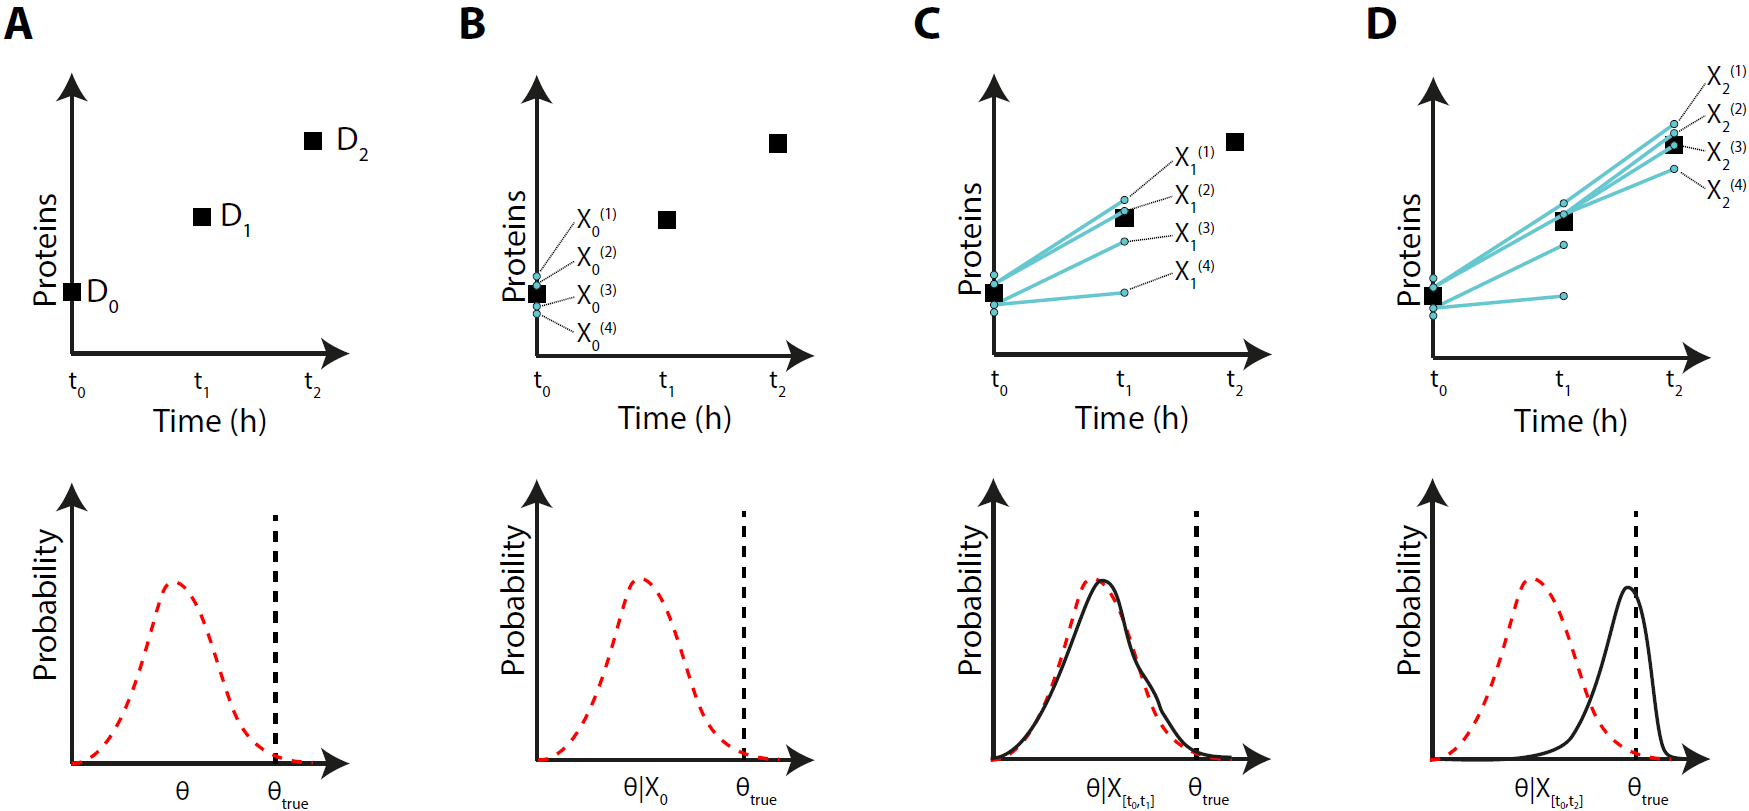
\includegraphics[height=2in]{figures/particle_filtering.png}
			~\footnote{Feigelman, 2016, Ph.D. Thesis}
		\end{center}
	\end{figure}
\end{frame}

\begin{frame}{Reaction Model}
	\begin{columns}
		\begin{column}{0.5\textwidth}
			\begin{itemize}
				\item Simple model in line with cross inhibiton assumption.
				\item Inhibiton modeled trough inverse michaelis menten kinetics.
				\item Parameterize production and degredation rates $k_i$ as well as inhibition contstant $K_Y$.
			\end{itemize}
		\end{column}
		\begin{column}{0.5\textwidth}  %%<--- here
    			\begin{center}
				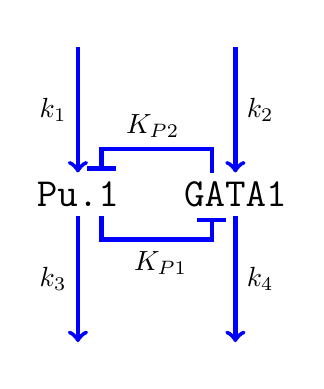
\begin{tikzpicture}[node distance=2cm]

\node (N0) {\Large $\varnothing$};
\node [right of = N0] (N1) {\Large $\varnothing$};
\node [below of = N0] (R0) {\Large \texttt{Pu.1}};
\node [below of = N1] (R1) {\Large \texttt{GATA1}};
\node [below of = R0] (N2) {\Large $\varnothing$};
\node [below of = R1] (N3) {\Large $\varnothing$};

\draw [->,ultra thick,blue] (N0) -- node[left, black] {$k_1$} (R0);
\draw [->,ultra thick,blue] (N1) -- node[right, black] {$k_2$} (R1);
\draw [->,ultra thick,blue] (R0) -- node[left, black] {$k_3$} (N2);
\draw [->,ultra thick,blue] (R1) -- node[right, black] {$k_4$} (N3);

\draw [-|,ultra thick,blue]
($ (R0) + (3mm,-2.75mm) $)
-- +(0,-3mm) 
-- +(0.75,-3mm) node[below, black]{$K_{P1}$}
-| ($ (R1) - (3mm,3mm) $) ;

\draw [-|,ultra thick,blue]
($ (R1) + (-3mm,2.75mm) $)
-- +(0,3mm) %node[above, black] {$v_3$}
-- +(-0.75,3mm) node[above, black]{$K_{P2}$}
-| ($ (R0) - (-3mm,-3mm) $);

				\end{tikzpicture}
     		\end{center}		
		\end{column}
	\end{columns}
	
	$$a_i = k_i \cdot (1 - \frac{X_i^{n}}{X_i^{n} + K_{Y}^{n}})$$
	
\end{frame}
	
\begin{frame}{Evaluation on synthetic data with known model}
	%\begin{figure}
		%\begin{tabular}{ccc}
  			%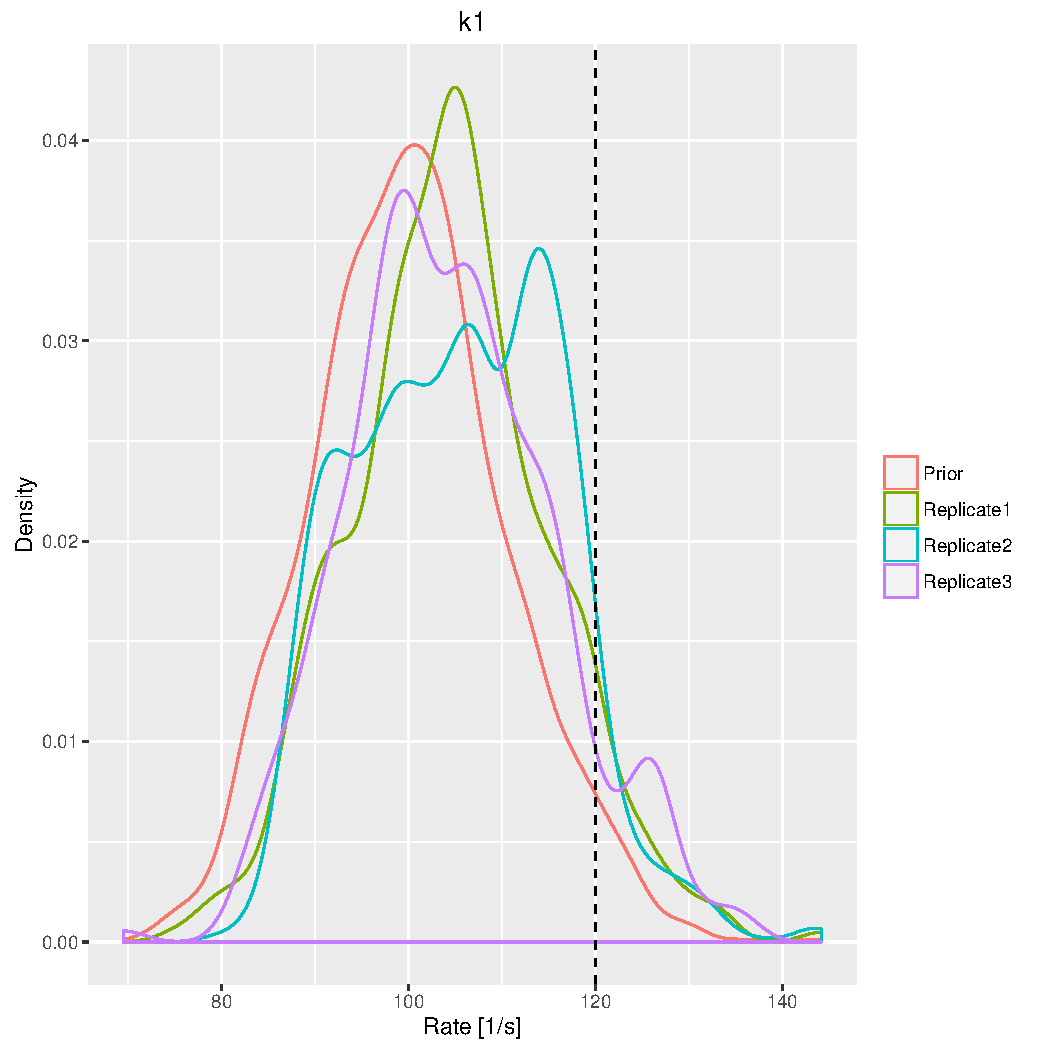
\includegraphics[width=1.3in]{figures/test_dist1.pdf} &   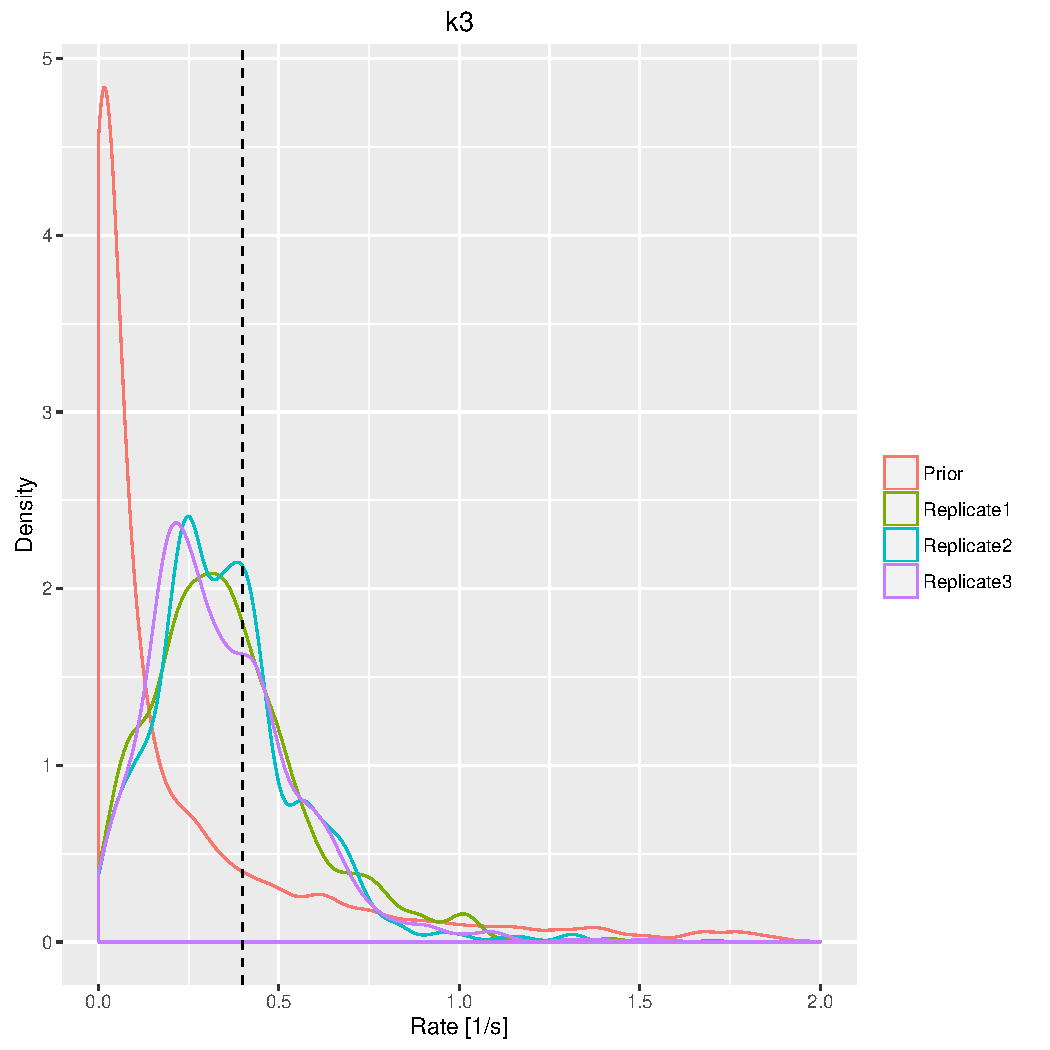
\includegraphics[width=1.3in]{figures/test_dist3.pdf}  & 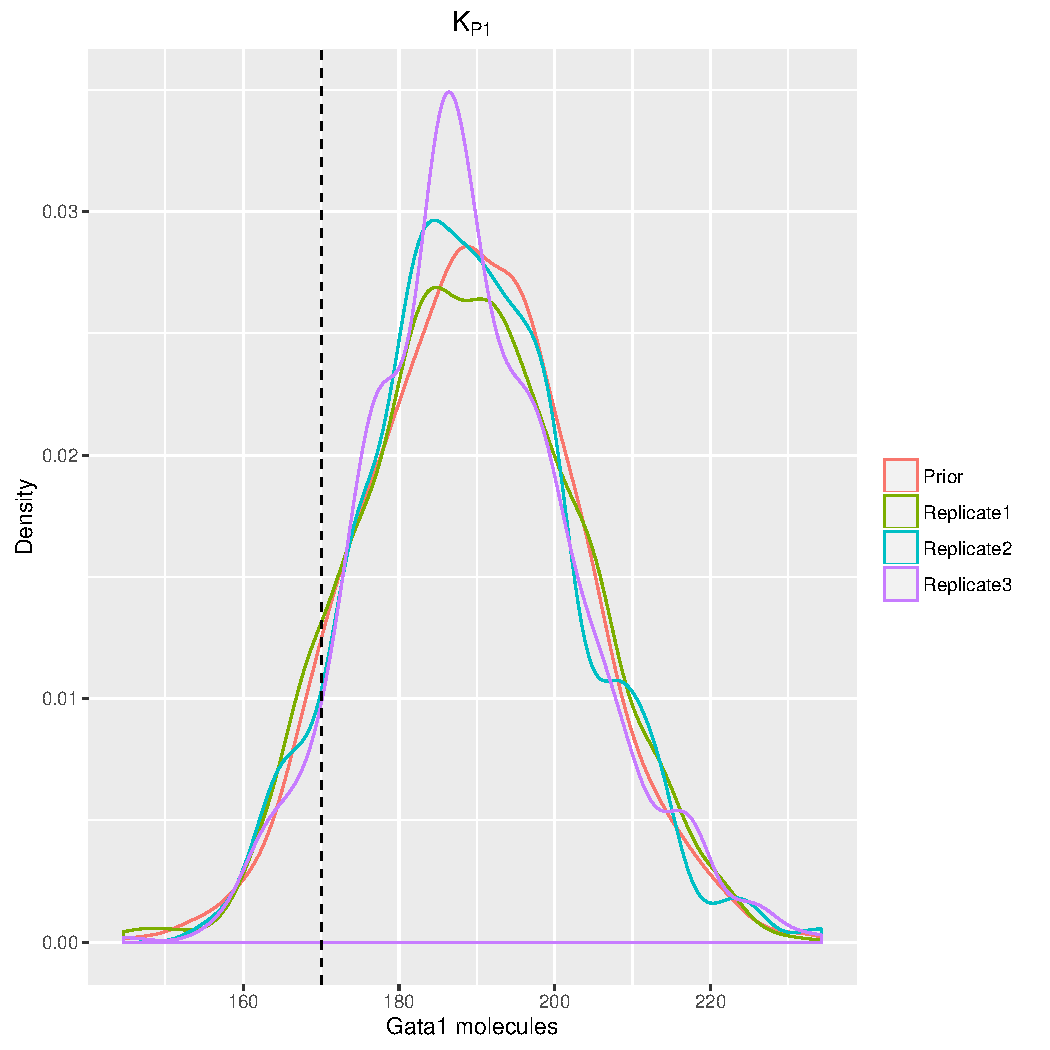
\includegraphics[width=1.3in]{figures/test_dist5.pdf}\\
 			%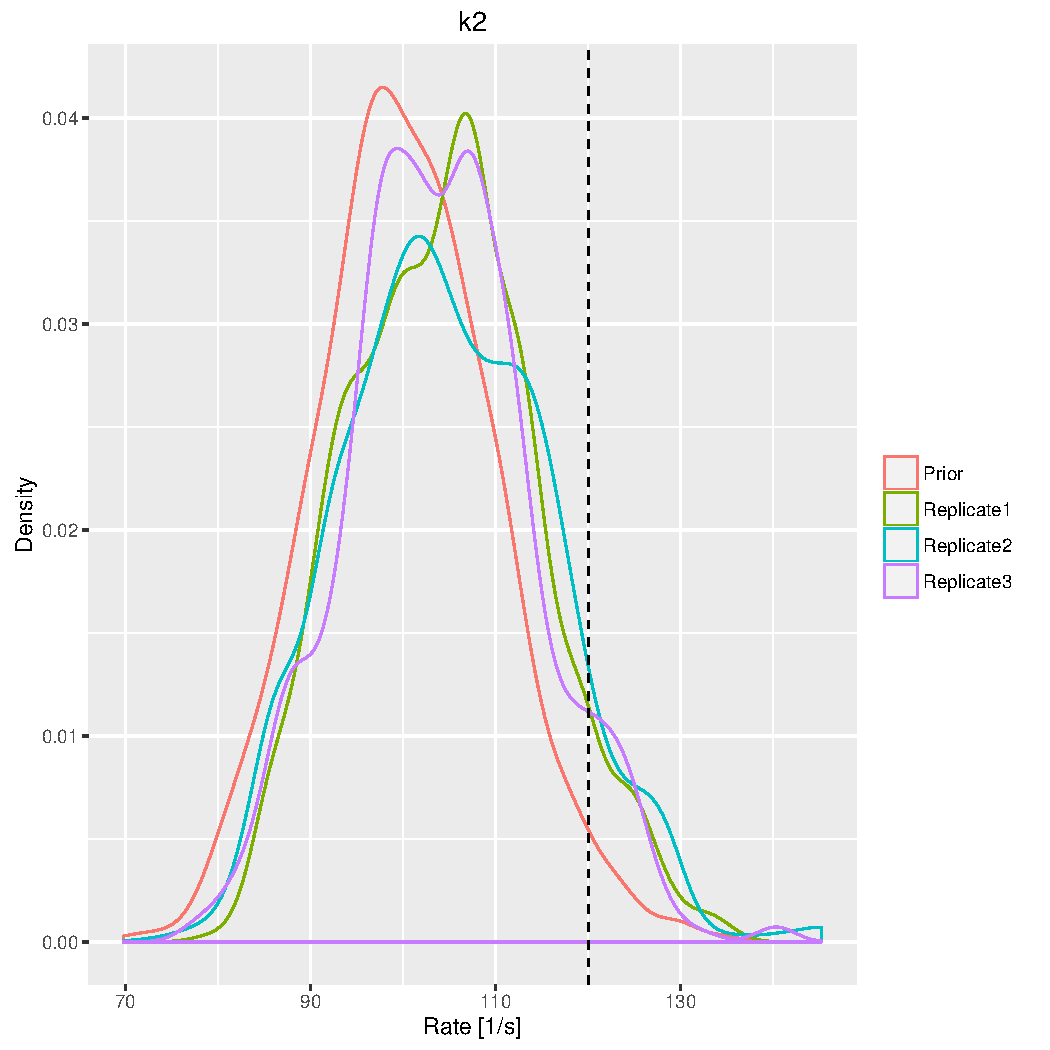
\includegraphics[width=1.3in]{figures/test_dist2.pdf} &   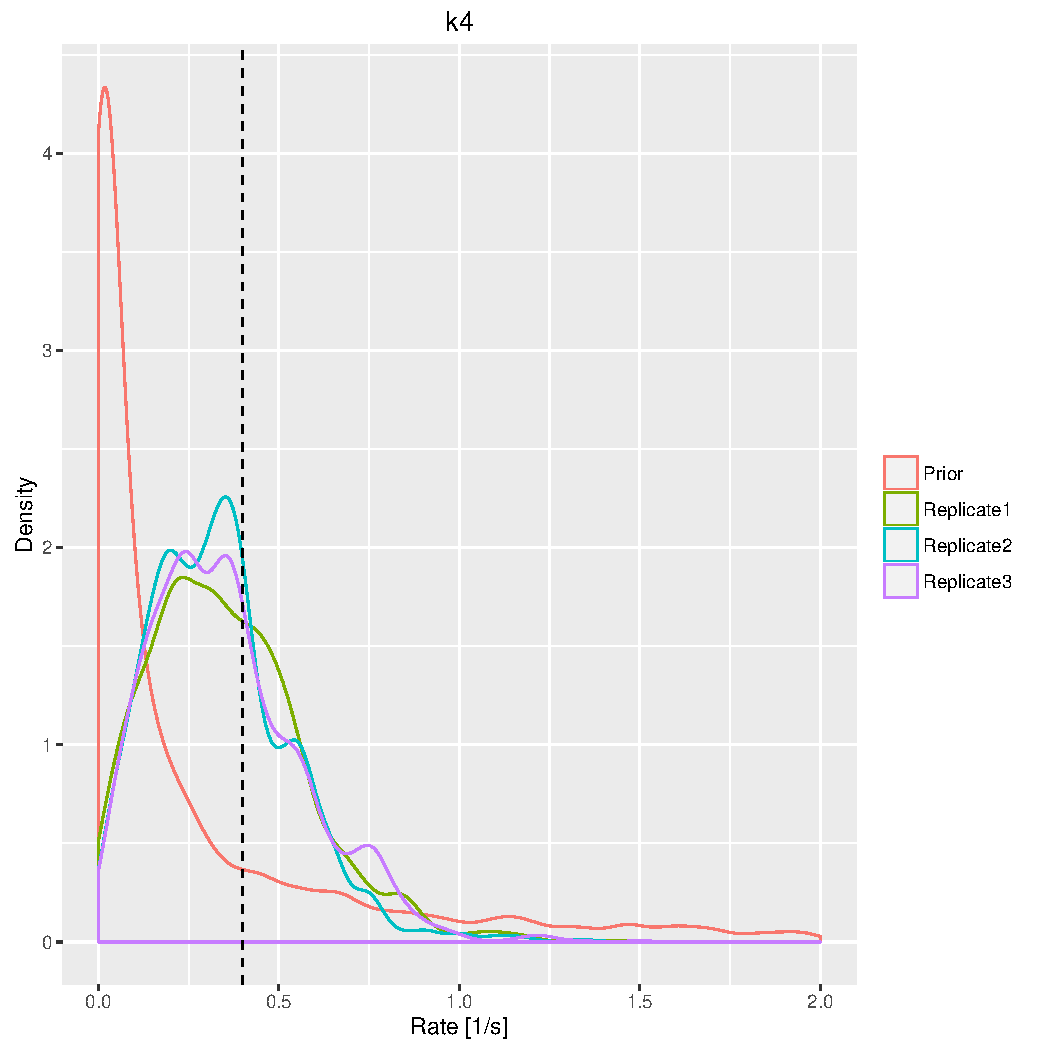
\includegraphics[width=1.3in]{figures/test_dist4.pdf}  & 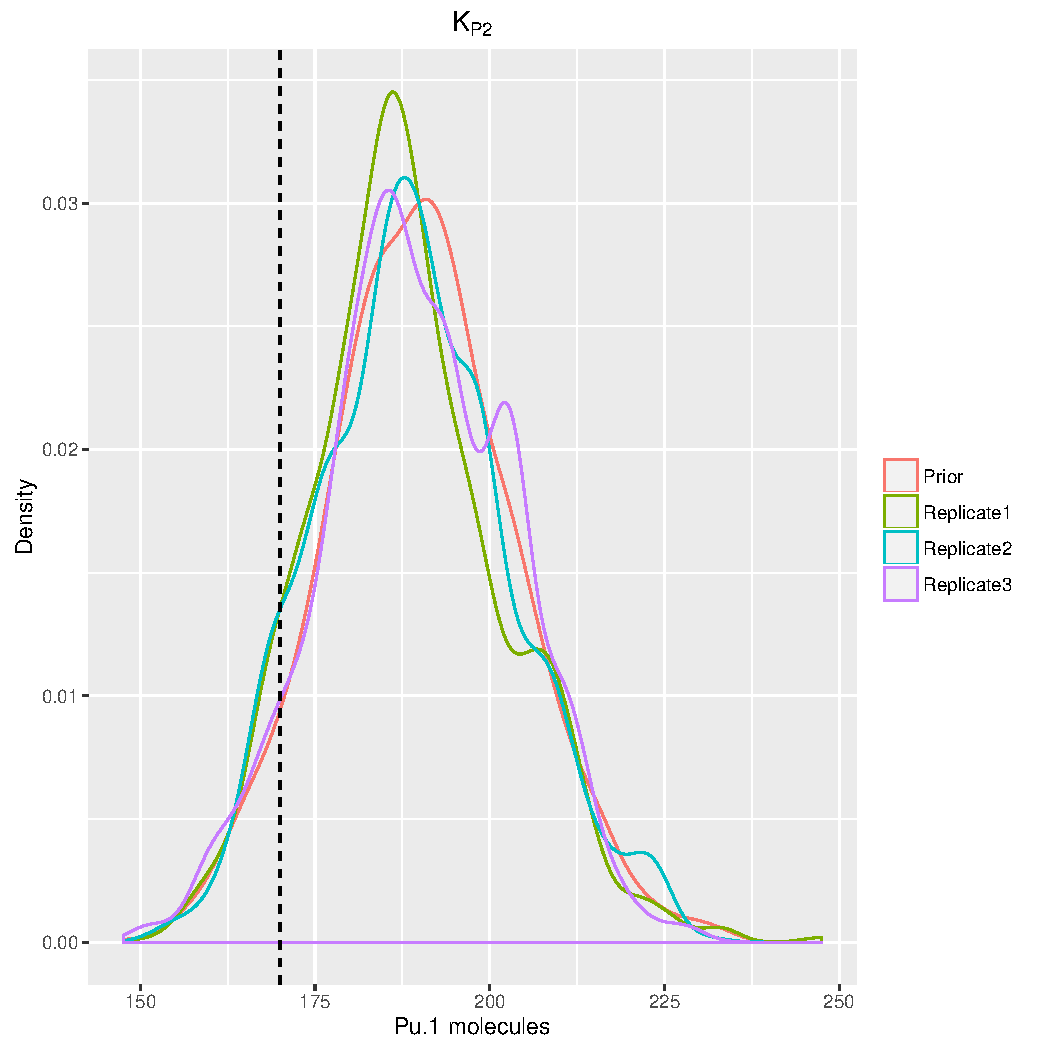
\includegraphics[width=1.3in]{figures/test_dist6.pdf}\\
		%\end{tabular}
	%\end{figure}

	\begin{figure}[ht]
		\begin{center}
			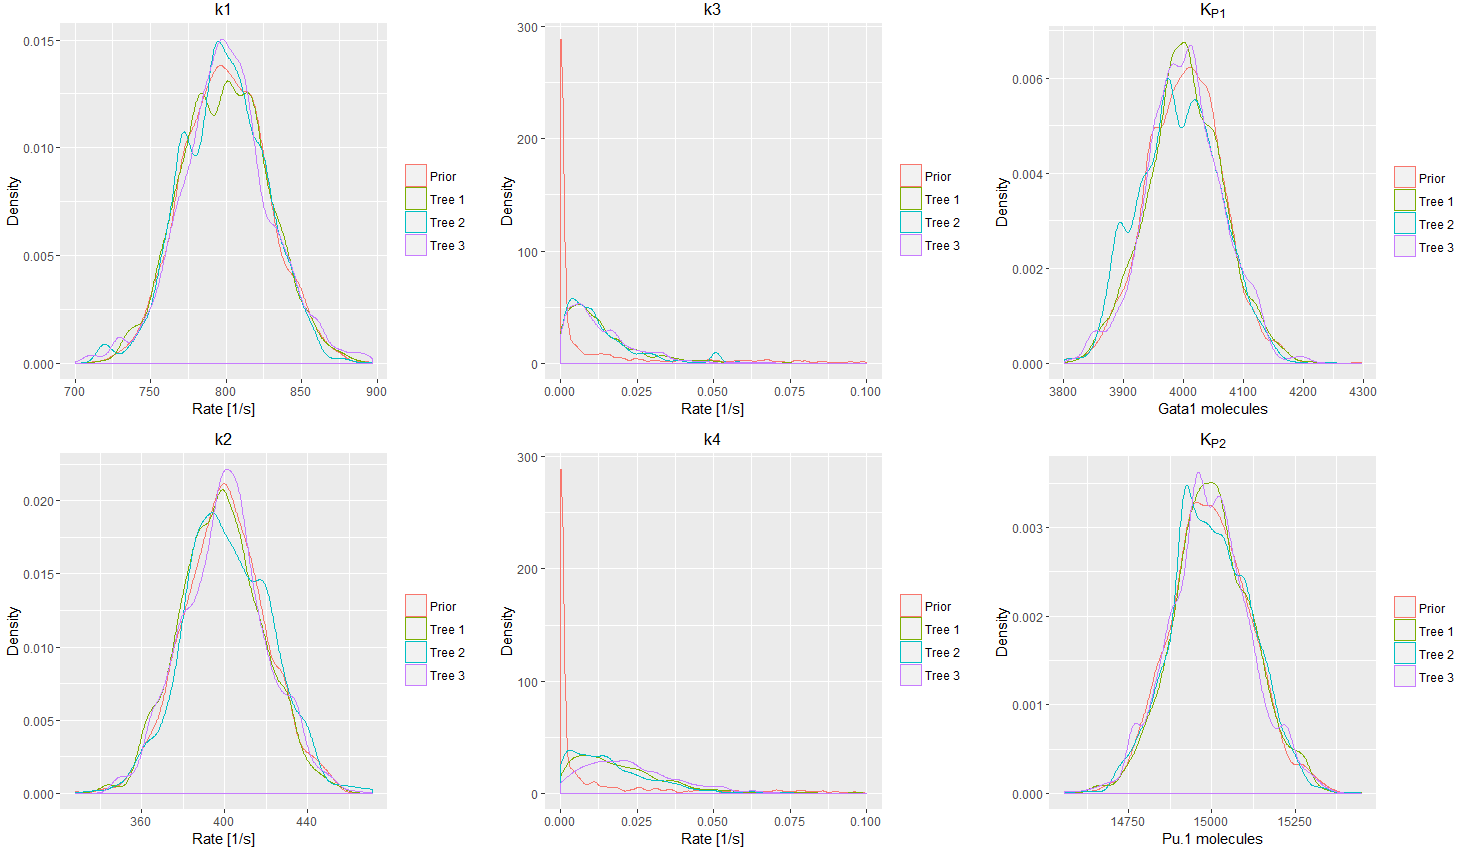
\includegraphics[height=2.1in]{figures/real_vertical.PNG}
		\end{center}
	\end{figure}
\end{frame}

\begin{frame}{Model Comparison}
	\begin{itemize}
		\item Compare performance of different models via Bayes Factors:
	\end{itemize}
	
	\begin{equation}
		B_{M1, M2} = \frac{P(M_1 | \mathcal{D})}{P(M_2 | \mathcal{D})}  \bayeseq \frac{P(M_1) P(\mathcal{D}| M_1)}{P(M_2) P(\mathcal{D} | M_2)} \label{eq:6}
	\end{equation}

	\begin{itemize}
		\item The average weight of the particle trajectories are used as Bayes Factor:
	\end{itemize}

	\begin{equation}
	P(\mathcal{D} | M) = P(\mathcal{D_0}) \prod_{l=1}^{N} P(\mathcal{D}_{i+1} | \mathcal{D}_{0:i}, M)\label{eq:7}
	\end{equation}

\end{frame}

\begin{frame}{Model Comparison}
		\begin{columns}
		\begin{column}{0.5\textwidth}
			\begin{itemize}
				\item Independent model used on synthetic data set.
				\item Model comparison by Bayes factors.
			\end{itemize}
		\end{column}
		\begin{column}{0.5\textwidth}  %%<--- here
    			\begin{center}
				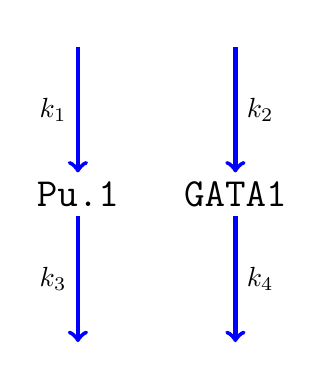
\begin{tikzpicture}[node distance=2cm]

\node (N0) {\Large $\varnothing$};
\node [right of = N0] (N1) {\Large $\varnothing$};
\node [below of = N0] (R0) {\Large \texttt{Pu.1}};
\node [below of = N1] (R1) {\Large \texttt{GATA1}};
\node [below of = R0] (N2) {\Large $\varnothing$};
\node [below of = R1] (N3) {\Large $\varnothing$};

\draw [->,ultra thick,blue] (N0) -- node[left, black] {$k_1$} (R0);
\draw [->,ultra thick,blue] (N1) -- node[right, black] {$k_2$} (R1);
\draw [->,ultra thick,blue] (R0) -- node[left, black] {$k_3$} (N2);
\draw [->,ultra thick,blue] (R1) -- node[right, black] {$k_4$} (N3);
				\end{tikzpicture}
     		\end{center}
		\end{column}
	\end{columns}
	\begin{equation}
	B_{M1, M2} = \frac{P(\mathcal{D} | M_{inhibitory})}{P(\mathcal{D} | M_{indepent})} = 			\frac{10^{-2221.498}}{10^{-2234.828}} \approx 2.14 \cdot 10^{13} \label{eq:8}
			\end{equation}
\end{frame}

\begin{frame}{Results on experiment data}
	\begin{figure}[ht]
		\begin{center}
			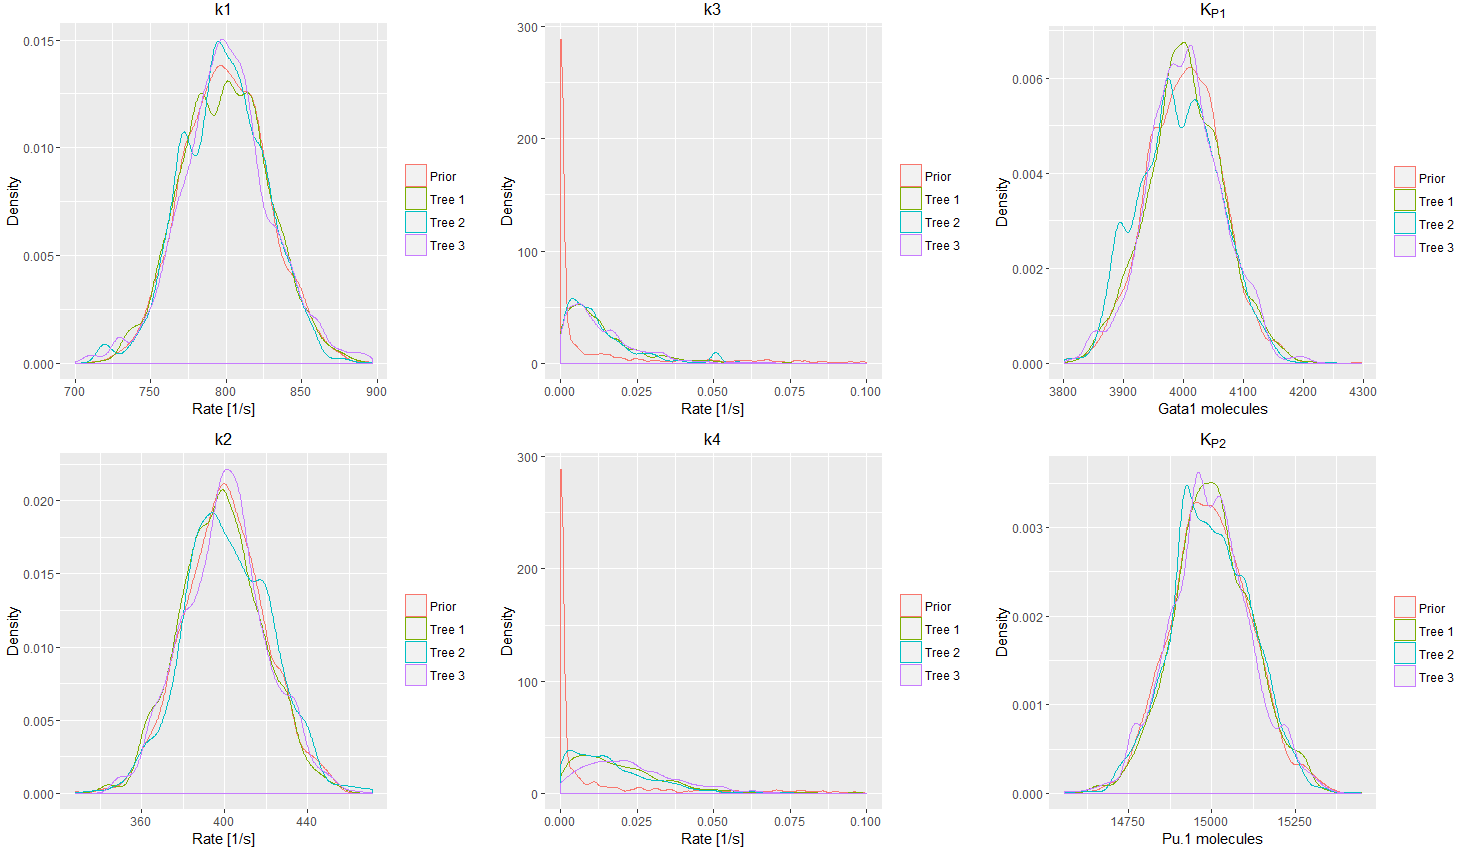
\includegraphics[height=2.1in]{figures/real_vertical.png}
		\end{center}
	\end{figure}
\end{frame}

\begin{frame}{Interpretation}
	\begin{itemize}
		\item Parameters of reaction model have varying susceptibility to fitting trough particle filtering.
		\item Model cannot accuratly describe the dynamic of the transcript factors.
		\item Recent finding (Hoppe et al., Nature, 2016) on the same data suggest the lineage choice to be independent from the transcription factor ratios.
		\item Particle filtering cannot infer the prescene of the external decision factor.
	\end{itemize}
\end{frame}

\begin{frame}{Conclusion \& Outlook}
	\begin{itemize}
		\item Particle filtering enable  the paramterization of models using time lapse data of cell lineage trees.
		\item Using the weight of particle trajectories models can be compared, allowing quantified comparison of theories.
		\item It would be interesting to know whether the decision process is really influenced by several latent factors under different reaction model.
	\end{itemize}
\end{frame}

\begin{frame}{References}

	\begin{itemize}
		\item Feigelman, J. (2016). "Stochastic and deterministic methods for the analysis of Nanog dynamics in mouse embryonic stem cells." PhD Thesis, Technische Universit\"at M\"unchen, Munich, Germany.
		\item Hoppe, P.S., Schwarzfischer, M., Loeffler, D.,  Kokkaliaris, K.D., Hilsenbeck, O., Mortz, N., ... \& Etzrodt, M. (2016). Early myeloid lineage choice is not initiated by random PU.1 to GATA1 protein ratios. \textit{Nature}, \textbf{535(7611)}, 299-302.
		\item Graf, T., \& Enver, T. (2009). Forcing cells to change lineages. \textit{Nature}, \textbf{462(7273)}, 587-594.
	\end{itemize}
\end{frame}


\end{document}
